\chapter{Resultados}
\label{chap:resultados}

Neste capítulo são apresentados e discutidos os resultados obtidos na realização do experimento descrito em detalhes no Capítulo \ref{chap:metodologia}. 
Será feita uma análise preliminar do conjunto de dados na seção \ref{sec:geral}.
Então, na seção \ref{sec:comparacao-algoritmos}, as métricas obtidas na execução dos algoritmos descritos anteriormente serão utilizados para avaliar a qualidade dos resultados.
Seguido então pela seção \ref{sec:subconjuntos}, que analisará métricas obtidas na aplicação dos algoritmos nos subconjuntos de dados discutidos na subseção \ref{subsec:subconjuntos}.
Gráficos \textit{SHAP} gerados na execução dos algoritmos serão analisados na seção \ref{sec:resultados-extras}, de forma a obter percepções sobre os resultados.

\section{Análise do Conjunto de Dados}
\label{sec:geral}

Antes de aplicar os algoritmos descritos anteriormente, é possível obter algumas informações do conjunto de dados. Existem 604.315 casos registrados, onde 94,91\% são casos leves e os restantes são considerados graves, destes, 25,15\% resultaram em óbito. Destes casos, embora o total seja de 43,5\% para o sexo masculino, eles consistem em 49,3\% dos casos graves. O sintoma mais comum foi a tosse, presente em 38\% de todos os casos e 72\% dos casos graves. Mapas de calor de correlação estão disponíveis nos apêndices \ref{apendice:correlacao}, \ref{apendice:correlacao-v0} e \ref{apendice:correlacao-v30}. As tabelas abaixo destrincham a distribuição da severidade dos casos e óbitos, de acordo com o Progresso de Vacinação e Idade.


  \begin{table}[H]
    \centering
    \begin{tabular}{|c|c|c|c|c|c|c|c|c|}
    \hline
    \textbf{Vacinação}          & \textbf{Total} & \textbf{\%} & \textbf{Leves} & \textbf{\%} & \textbf{Graves} & \textbf{\%} & \textbf{Óbitos} & \textbf{\%} \\ \hline
    \textbf{=0\%}               & 272144         & 45.64\%           & 251882         & 91.03\%           & 15689           & 5.67\%             & 4573            & 1.65\%             \\ \hline
    \textbf{\textgreater{}0\%}  & 332171         & 54.97\%           & 321697         & 95.93\%           & 7315            & 2.18\%             & 3159            & 0.94\%             \\ \hline
    \textbf{\textgreater{}15\%} & 260258         & 43.07\%           & 252035         & 95.93\%           & 5749            & 2.19\%             & 2474            & 0.94\%             \\ \hline
    \textbf{\textgreater{}30\%} & 188579         & 31.21\%           & 182667         & 95.95\%           & 4118            & 2.16\%             & 1794            & 0.94\%             \\ \hline
    \textbf{\textgreater{}45\%} & 112003         & 18.53\%           & 108533         & 95.97\%           & 2381            & 2.11\%             & 1089            & 0.96\%             \\ \hline
    \textbf{\textgreater{}60\%} & 36072          & 5.97\%            & 34891          & 95.76\%           & 816             & 2.24\%             & 365             & 1.00\%             \\ \hline
    \end{tabular}
    \caption{Quantidade de casos leves, graves e óbitos por progresso de vacinação}
    \label{tbl:tabela-vacina-severidade}
    \end{table}
    
\begin{table}[H]
  \centering
  \begin{tabular}{|c|c|c|c|c|c|c|}
  \hline
  \textbf{Idade} & \textbf{Leves} & \textbf{\%} & \textbf{Graves} & \textbf{\%} & \textbf{Óbitos} & \textbf{\%} \\ \hline
  \textbf{0-9}   & 21260          & 89.68\%           & 2365            & 9.98\%             & 41              & 0.17\%             \\ \hline
  \textbf{10-19} & 36142          & 98.63\%           & 465             & 1.27\%             & 19              & 0.05\%             \\ \hline
  \textbf{20-29} & 107641         & 98.27\%           & 1702            & 1.55\%             & 96              & 0.09\%             \\ \hline
  \textbf{30-39} & 130232         & 97.02\%           & 3457            & 2.58\%             & 272             & 0.20\%             \\ \hline
  \textbf{40-49} & 111150         & 95.68\%           & 3882            & 3.34\%             & 570             & 0.49\%             \\ \hline
  \textbf{50-59} & 83865          & 92.95\%           & 3979            & 4.41\%             & 1191            & 1.32\%             \\ \hline
  \textbf{60-69} & 51814          & 88.49\%           & 3145            & 5.37\%             & 1796            & 3.07\%             \\ \hline
  \textbf{70-79} & 22328          & 79.54\%           & 2224            & 7.92\%             & 1760            & 6.27\%             \\ \hline
  \textbf{80+}   & 9147           & 61.25\%           & 1758            & 11.77\%            & 2014            & 13.49\%            \\ \hline
  \end{tabular}
  \caption{Quantidade de casos leves, graves e óbitos por idade}
  \label{tbl:tabela-idade-severidade}
  \end{table}

As figuras \ref{fig:plot-sev} e \ref{fig:plot-obt} comparam a distribuição da porcentagem de casos graves e óbitos, respectivamente, pelas categorias de idade e progresso da vacinação.

\begin{figure}[ht!]
  \centering
  \fcolorbox{white}{white}{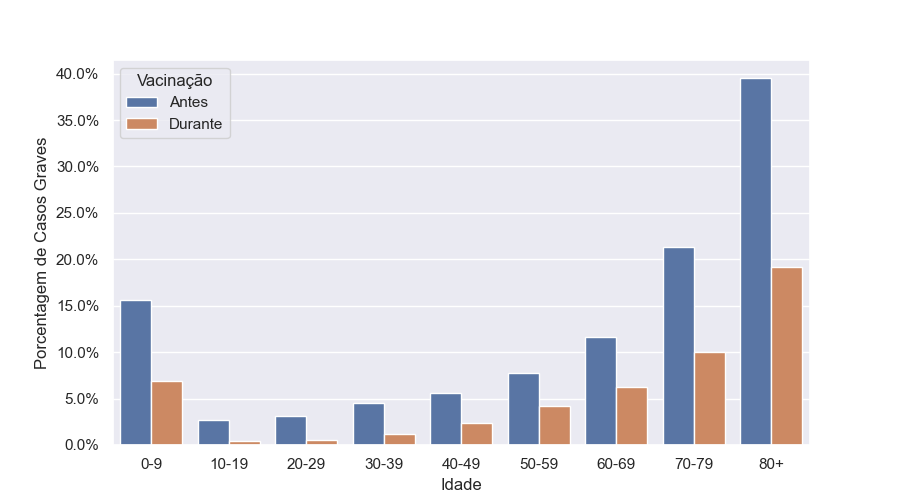
\includegraphics[width=0.65\textwidth]{chapters/resultados/images/plot_idade_severidade_vacina.png}}
  \caption{\textmd{Gráfico da porcentagem de casos graves para idades e vacinação}}
  \label{fig:plot-sev}
\end{figure}

\begin{figure}[ht!]
  \centering
  \fcolorbox{white}{white}{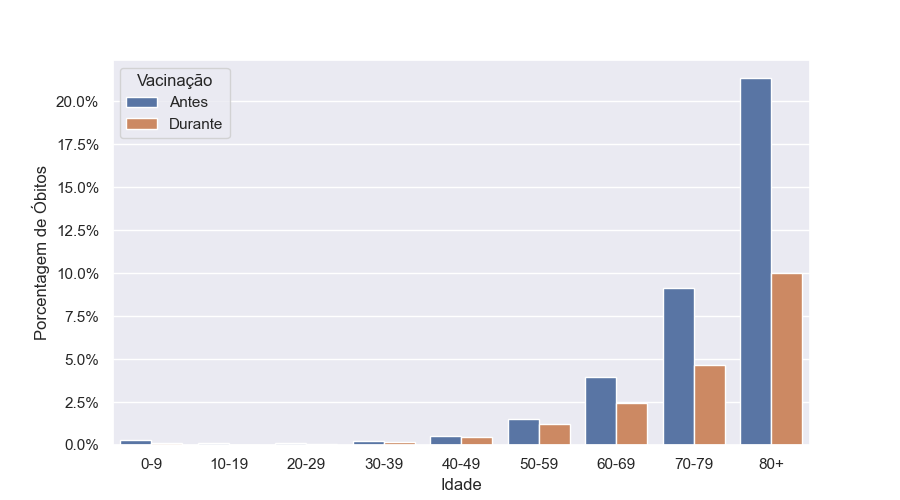
\includegraphics[width=0.65\textwidth]{chapters/resultados/images/plot_idade_obito_vacina.png}}
  \caption{\textmd{Gráfico da porcentagem de óbitos para idades e vacinação}}
  \label{fig:plot-obt}
\end{figure}



\section{Comparação entre Algoritmos}
\label{sec:comparacao-algoritmos}

Após uma certa quantidade de iterações do processo de otimização de parâmetros como especificado na subseção \ref{subsec:otimizacao}, os modelos gerados pelos algoritmos de classificação \textit{k-Nearest Neighbors} (kNN), \textit{Decision Tree} (DT), \textit{Random Forest} (RF), \textit{Gradient Boosting} (GB), \textit{Light Gradient Boosting} (LGB) e \textit{XGBoost} (XGB) %e \textit{Neural Network} (NN)% 
na etapa de treinamento foram aplicados no conjunto de dados de teste.

Cada algoritmo foi executado 20 vezes, aleatorizando o conjunto de dados em cada uma delas, coletando então suas métricas de acurácia, precisão, sensibilidade, \textit{F1-Score} e \textit{AUC-ROC} para cada execução. 
Como discutido na subseção \ref{subsec:calculo-metricas}, as métricas macro representam a média dos resultados de cada classe, que neste conjunto de dados são casos leves e casos graves. 
A média e desvio padrão de cada métrica foi calculada, e as métricas consideradas relevantes para comparação se encontram na tabela \ref{tab:comparacao-algoritmos-normal}, onde o maior valor para cada uma está representado em negrito.

\begin{table}[H]
  \footnotesize
  \centering
  \begin{tabular}{l|c|c|c|c|c|}
  \cline{2-6}
  \textbf{}                          & \textbf{Acurácia}      & \textbf{Precisão Macro} & \textbf{Sensib. Macro} & \textbf{F1-Score Macro} & \textbf{AUC-ROC}       \\ \hline
  \multicolumn{1}{|l|}{\textbf{kNN}} & 0,9790±0,0001          & 0,9475±0,0007           & 0,8228±0,0020          & 0,8739±0,0011           & 0,8228±0,0020          \\ \hline
  \multicolumn{1}{|l|}{\textbf{DT}}  & 0,9767±0,0015          & 0,9558±0,0133           & 0,7913±0,0094          & 0,8534±0,0101           & 0,7913±0,0094          \\ \hline
  \multicolumn{1}{|l|}{\textbf{RF}}  & 0,9828±0,0001          & \textbf{0,9795±0,0006}  & 0,8395±0,0012          & 0,8962±0,0009           & 0,8395±0,0012          \\ \hline
  \multicolumn{1}{|l|}{\textbf{GB}}  & 0,9835±0,0002          & 0,9727±0,0022           & 0,8513±0,0015          & 0,9020±0,0012           & 0,8513±0,0015          \\ \hline
  \multicolumn{1}{|l|}{\textbf{LGB}} & 0,9835±0,0002          & 0,9748±0,0016           & 0,8498±0,0015          & 0,9018±0,0001           & 0,8498±0,0015          \\ \hline
  \multicolumn{1}{|l|}{\textbf{XGB}} & \textbf{0,9838±0,0003} & 0,9707±0,0010           & \textbf{0,8571±0,0031} & \textbf{0,9052±0,0022}  & \textbf{0,8571±0,0031} \\ \hline 
\end{tabular}
\caption{Médias de métricas de algoritmos de classificação na etapa de teste}
\label{tab:comparacao-algoritmos-normal}
\end{table}

Levando em consideração a métrica \textit{AUC-ROC} como métrica de avaliação, é possível observar que, enquanto todos os algoritmos alcançaram um valor próximo ou acima de 80\%, o algoritmo \textit{XGBoost} obteve o melhor desempenho, bem próximo dos outros algoritmos de \textit{Gradient Boosting}. O \textit{F1-Score Macro} também é um indicador de desempenho satisfatório, e todos os algoritmos alcançaram valores acima de 85\%, com os algoritmos baseados em \textit{Gradient Boosting} alcançando valores acima de 90\%. 

Embora a Precisão Macro tenha alcançado valores altos, até acima de 97\%, a Sensibilidade Macro ficou sempre abaixo dos 90\%, devido a uma quantidade considerável de falsos negativos, casos graves classificados como leves. É possível observar este resultado na tabela \ref{tab:matriz-confusao-xgboost}, que mostra a matriz de confusão do \textit{XGBoost} com melhor \textit{F1-Score} das 20 execuções, 90,97\%.

\begin{table}[H]
  \footnotesize
  \centering
  \centering
  \begin{tabular}{l|c|c|}
    \cline{2-3}
    \textbf{}                         & \multicolumn{1}{l|}{\textbf{Predição: LEVE}} & \multicolumn{1}{l|}{\textbf{Predição: GRAVE}} \\ \hline
    \multicolumn{1}{|l|}{\textbf{Real: LEVE}}  & 114511                                       & 205 (0,18\%)                                           \\ \hline
    \multicolumn{1}{|l|}{\textbf{Real: GRAVE}} & 1664 (27,07\%)                                         & 4483                                          \\ \hline   
  \end{tabular}
  \caption{Matriz de confusão de uma execução do \textit{XGBoost}}
  \label{tab:matriz-confusao-xgboost}
\end{table}

Tomando a tabela \ref{tab:matriz-confusao-xgboost} como exemplo, somente 0,18\% de casos leves foram preditos como graves, um número ínfimo de falsos negativos. Isso significa que existe uma confiabilidade satisfatória nos casos preditos como graves. 

Contudo, 27\% dos casos graves foram erroneamente preditos como leves, significando que cerca de 1/4 dos casos graves não foram percebidos pelo algoritmo. Este fenômeno se mostrou presente em todos os algoritmos analisados, sendo a causa da diminuição da Sensibilidade Macro observada na tabela \ref{tab:comparacao-algoritmos-normal}.

Este problema ocorre devido ao desbalanceamento do conjunto de dados, onde existem 20x mais casos leves que graves. Portanto, durante a etapa de otimização de parâmetros descrita na subseção \ref{subsec:otimizacao}, técnicas de balanceamento de dados foram utilizadas. O processo de balanceamento consiste em igualar a quantidade de classes no conjunto de dados, excluindo registros aleatórios da classe mais comum. Os resultados se encontram na tabela \ref{tab:comparacao-algoritmos-undersample}.

\begin{table}[H]
  \footnotesize
  \centering
  \begin{tabular}{l|c|c|c|c|c|}
  \cline{2-6}
  \textbf{}                          & \textbf{Acurácia}      & \textbf{Precisão Macro} & \textbf{Sensib. Macro} & \textbf{F1-Score Macro} & \textbf{AUC-ROC}       \\ \hline
  \multicolumn{1}{|l|}{\textbf{kNN}} & 0,9047±0,0027          & 0,9050±0,0026           & 0,9047±0,0027          & 0,9047±0,0027           & 0,9047±0,0027          \\ \hline
  \multicolumn{1}{|l|}{\textbf{DT}}  & 0,8896±0,0102          & 0,8905±0,0096           & 0,8896±0,0102          & 0,8895±0,0103           & 0,8896±0,0102          \\ \hline
  \multicolumn{1}{|l|}{\textbf{RF}}  & 0,9150±0,0019          & 0,9158±0,0020           & 0,9150±0,0019          & 0,9150±0,0019           & 0,9150±0,0019          \\ \hline
  \multicolumn{1}{|l|}{\textbf{GB}}  & 0,9234±0,0022          & 0,9238±0,0022           & 0,9234±0,0022          & 0,9234±0,0022           & 0,9234±0,0022          \\ \hline
  \multicolumn{1}{|l|}{\textbf{LGB}} & 0,9233±0,0009          & 0,9239±0,0009           & 0,9233±0,0009          & 0,9233±0,0009           & 0,9233±0,0009          \\ \hline
  \multicolumn{1}{|l|}{\textbf{XGB}} & \textbf{0,9243±0,0016} & \textbf{0,9249±0,0013}  & \textbf{0,9243±0,0016} & \textbf{0,9242±0,0016}  & \textbf{0,9243±0,0016} \\ \hline
\end{tabular}
\caption{Médias de métricas de algoritmos de classificação na etapa de testes com classes balanceadas}
\label{tab:comparacao-algoritmos-undersample}
\end{table}

A Sensibilidade Macro teve um aumento considerável, chegando acima dos 90\% na maioria dos algoritmos, enquanto a Precisão Macro sofreu uma queda. O \textit{F1-Score} consequentemente teve um aumento, por ser a média harmônica dessas medidas. A acurácia caiu significativamente, não mais inflada pelos casos leves, enquanto o valor \textit{AUC-ROC} cresceu proporcionalmente. Demonstram-se essas diferenças mais detalhadamente na tabela \ref{tab:matriz-confusao-xgboost-undersample}, uma matriz de confusão do XGBoost com \textit{F1-Score} de 92,67\%.

\begin{table}[H]
  \footnotesize
  \centering
  \centering
  \begin{tabular}{l|c|c|}
    \cline{2-3}
    \textbf{}                         & \multicolumn{1}{l|}{\textbf{Predição: LEVE}} & \multicolumn{1}{l|}{\textbf{Predição: GRAVE}} \\ \hline
    \multicolumn{1}{|l|}{\textbf{Real: LEVE}}  & 5770                                       & 377 (6,13\%)                                           \\ \hline
    \multicolumn{1}{|l|}{\textbf{Real: GRAVE}} & 524 (8,52\%)                                         & 5623                                          \\ \hline   
  \end{tabular}
  \caption{Matriz de confusão de uma execução do \textit{XGBoost} com classes balanceadas}
  \label{tab:matriz-confusao-xgboost-undersample}
\end{table}

Neste cenário, a diferença entre a proporção de falsos positivos e falsos negativos se equilibra, ainda que se mantenha maior nos casos graves. Existe uma chance de que casos leves sejam preditos como graves, mas a chance de que casos graves sejam preditos como leves é muito menor que anteriormente. Considerando a natureza médica do problema, uma menor taxa de casos graves perdidos pode ser considerada uma melhoria significativa, mesmo que exista um aumento na quantidade de alarmes falsos para casos leves \cite{medical-ai-measure}. Portanto, assimilando este julgamento ao aumento do valor \textit{AUC-ROC}, escolhido como métrica de desempenho, balancear o conjunto de dados por \textit{RandomUnderSampler} se evidencia como uma melhoria.


\section{Comparação entre Algoritmos em Subconjuntos}
\label{sec:subconjuntos}

Como discutido na subseção \ref{subsec:subconjuntos}, a aplicação de certos filtros no conjunto de dados permite observar diferentes cenários, que podem trazer novas percepções ao problema. Sendo assim, os algoritmos foram utilizados em subconjuntos de dados, para obter métricas que podem ser comparadas entre eles. As métricas foram obtidas usando os mesmos métodos que as métricas da seção \ref{sec:comparacao-algoritmos}, tendo o conjunto de dados balanceado por \textit{RandomUnderSampler}. Gráficos \textit{SHAP} gerados na execução dos algoritmos serão analisados e discutidos na seção \ref{sec:resultados-extras}.

\subsection{Omitindo Dados Sintomáticos}
\label{subsec:subconjuntos-sem-sintomas}

Remover as colunas de dados sintomáticos permite observar como os algoritmos predizem os casos leves e graves se baseando somente nos dados demográficos, doenças preexistentes e progresso da vacinação.

\begin{table}[H]
  \footnotesize
  \centering
  \begin{tabular}{l|c|c|c|c|c|}
  \cline{2-6}
  \textbf{}                          & \textbf{Acurácia}      & \textbf{Precisão Macro} & \textbf{Sensib. Macro} & \textbf{F1-Score Macro} & \textbf{AUC-ROC}       \\ \hline
  \multicolumn{1}{|l|}{\textbf{kNN}} & 0,7125±0,0162          & 0,7144±0,0172           & 0,7125±0,0162          & 0,7119±0,0159           & 0,7125±0,0162          \\ \hline
  \multicolumn{1}{|l|}{\textbf{DT}}  & 0,7383±0,0051          & 0,7415±0,0036           & 0,7383±0,0051          & 0,7375±0,0056           & 0,7383±0,0051          \\ \hline
  \multicolumn{1}{|l|}{\textbf{RF}}  & 0,7383±0,0025          & 0,7402±0,0029           & 0,7383±0,0025          & 0,7378±0,0024           & 0,7383±0,0025          \\ \hline
  \multicolumn{1}{|l|}{\textbf{GB}}  & \textbf{0,7463±0,0044} & \textbf{0,7481±0,0042}  & \textbf{0,7463±0,0044} & \textbf{0,7459±0,0045}  & \textbf{0,7463±0,0044} \\ \hline
  \multicolumn{1}{|l|}{\textbf{LGB}} & 0,7453±0,0019          & 0,7470±0,0019           & 0,7453±0,0019          & 0,7448±0,0019           & 0,7453±0,0019          \\ \hline
  \multicolumn{1}{|l|}{\textbf{XGB}} & 0,7451±0,0047          & 0,7470±0,0045           & 0,7451±0,0047          & 0,7446±0,0047           & 0,7451±0,0047          \\ \hline
  \end{tabular}
\caption{Comparação de algoritmos sem dados sintomáticos}
\label{tab:comparacao-sem-dados-sintomaticos}
\end{table}

A tabela \ref{tab:comparacao-sem-dados-sintomaticos} apresenta as métricas da aplicação dos algoritmos nos subconjuntos de dados sem dados sintomáticos. É possível perceber uma queda em todas as métricas, consistente entre os algoritmos, devido à importância dos dados sintomáticos no julgamento. Todos os valores do \textit{Gradient Boosting} se mantêm em torno dos 75\%, incluindo o \textit{AUC-ROC}, utilizado como métrica de desempenho, com uma queda média de 18\% comparado à sua execução no conjunto de dados completo. Com isso, embora menos precisos, é possível considerar válida a aplicação dos algoritmos nos subconjuntos de dados sem dados sintomáticos.



\subsection{Prevendo Óbitos}
\label{subsec:subconjuntos-com-morte}

Separando o conjunto de dados entre casos leves ou graves e óbitos, é possível observar como os algoritmos predizem óbito do paciente de acordo com seus dados demográficos, sintomas, doenças preexistentes e progresso da vacinação.

\begin{table}[H]
  \footnotesize
  \centering
  \begin{tabular}{l|c|c|c|c|c|}
    \cline{2-6}
    \textbf{}                          & \textbf{Acurácia}      & \textbf{Precisão Macro} & \textbf{Sensib. Macro} & \textbf{F1-Score Macro} & \textbf{AUC-ROC}       \\ \hline
    \multicolumn{1}{|l|}{\textbf{kNN}} & 0,9354±0,0060          & 0,9356±0,0059           & 0,9354±0,0060          & 0,9354±0,0060           & 0,9354±0,0060          \\ \hline
    \multicolumn{1}{|l|}{\textbf{DT}}  & 0,9228±0,0069          & 0,9231±0,0067           & 0,9228±0,0069          & 0,9227±0,0069           & 0,9228±0,0069          \\ \hline
    \multicolumn{1}{|l|}{\textbf{RF}}  & 0,9435±0,0044          & 0,9435±0,0044           & 0,9435±0,0044          & 0,9435±0,0044           & 0,9435±0,0044          \\ \hline
    \multicolumn{1}{|l|}{\textbf{GB}}  & 0,9499±0,0038          & 0,9499±0,0038           & 0,9499±0,0038          & 0,9499±0,0038           & 0,9499±0,0038          \\ \hline
    \multicolumn{1}{|l|}{\textbf{LGB}} & 0,9465±0,0027          & 0,9465±0,0027           & 0,9465±0,0027          & 0,9465±0,0027           & 0,9465±0,0027          \\ \hline
    \multicolumn{1}{|l|}{\textbf{XGB}} & \textbf{0,9547±0,0057} & \textbf{0,9547±0,0057}  & \textbf{0,9547±0,0057} & \textbf{0,9547±0,0057}  & \textbf{0,9547±0,0057} \\ \hline
    \end{tabular}
\caption{Comparação de algoritmos prevendo óbito}
\label{tab:comparacao-obito}
\end{table}

A tabela \ref{tab:comparacao-obito} apresenta as métricas da aplicação dos algoritmos nos subconjuntos de dados de óbito.
Neste caso, todos os algoritmos alcançaram métricas acima de 92\%, sendo o \textit{XGBoost} o único que alcançou uma média acima de 95\%, mais preciso que no conjunto de dados completo. Acredita-se que isso ocorre devido a melhor separação das classes.

Similar ao discutido na subseção \ref{subsec:subconjuntos-sem-sintomas}, é possível observar como os algoritmos predizem óbito do paciente sem os sintomas, usando seus dados demográficos, doenças preexistentes e progresso da vacinação.

\begin{table}[H]
  \footnotesize
  \centering
  \begin{tabular}{l|c|c|c|c|c|}
    \cline{2-6}
    \textbf{}                          & \textbf{Acurácia}      & \textbf{Precisão Macro} & \textbf{Sensib. Macro} & \textbf{F1-Score Macro} & \textbf{AUC-ROC}       \\ \hline
    \multicolumn{1}{|l|}{\textbf{kNN}} & 0,8450±0,0069          & 0,8460±0,0066           & 0,8450±0,0069          & 0,8449±0,0070           & 0,8450±0,0069          \\ \hline
    \multicolumn{1}{|l|}{\textbf{DT}}  & 0,8468±0,0094          & 0,8475±0,0091           & 0,8468±0,0094          & 0,8467±0,0095           & 0,8468±0,0094          \\ \hline
    \multicolumn{1}{|l|}{\textbf{RF}}  & 0,8473±0,0036          & 0,8476±0,0036           & 0,8473±0,0036          & 0,8473±0,0036           & 0,8473±0,0036          \\ \hline
    \multicolumn{1}{|l|}{\textbf{GB}}  & 0,8598±0,0021          & 0,8601±0,0022           & 0,8598±0,0021          & 0,8598±0,0021           & 0,8598±0,0021          \\ \hline
    \multicolumn{1}{|l|}{\textbf{LGB}} & 0,8554±0,0030          & 0,8557±0,0028           & 0,8554±0,0030          & 0,8553±0,0030           & 0,8554±0,0030          \\ \hline
    \multicolumn{1}{|l|}{\textbf{XGB}} & \textbf{0,8597±0,0050} & \textbf{0,8602±0,0051}  & \textbf{0,8597±0,0050} & \textbf{0,8596±0,0050}  & \textbf{0,8597±0,0050} \\ \hline
    \end{tabular}
\caption{Comparação de algoritmos prevendo óbito sem dados sintomáticos}
\label{tab:comparacao-obito-sem-dados-sintomaticos}
\end{table}

A tabela \ref{tab:comparacao-obito-sem-dados-sintomaticos} apresenta as métricas da aplicação dos algoritmos nos subconjuntos de dados de óbito com dados sintomáticos omitidos. As métricas se mantêm em torno de 85\%, tendo um aumento se comparado à predição de casos leves e graves sem os dados sintomáticos. É possível considerar satisfatório aplicar os algoritmos de classificação na predição de óbito do paciente somente usando seus dados demográficos, doenças preexistentes e progresso da vacinação.


\subsection{Filtrando por Progresso de Vacinação}
\label{subsec:subconjuntos-vacinacao}

Filtrando o conjunto de dados por progresso de vacinação, é possível observar possíveis mudanças no perfil de risco dos pacientes em casos leves e graves. Esta abordagem foi então aplicada no conjunto de dados completo e no subconjunto de dados de óbito.


\subsubsection{Casos antes da vacina}
\label{subsub:comparacao-antes-vacina}

\begin{table}[H]
  \footnotesize
  \centering
  \begin{tabular}{l|c|c|c|c|c|}
    \cline{2-6}
    \multicolumn{1}{c|}{\textbf{}}     & \textbf{Acurácia}      & \textbf{Precisão Macro} & \textbf{Sensib. Macro} & \textbf{F1-Score Macro} & \textbf{AUC-ROC}       \\ \hline
    \multicolumn{1}{|l|}{\textbf{kNN}} & 0.8557±0.0053          & 0.8571±0.0055           & 0.8557±0.0053          & 0.8555±0.0053           & 0.8557±0.0053          \\ \hline
    \multicolumn{1}{|l|}{\textbf{DT}}  & 0.8433±0.0099          & 0.8456±0.0102           & 0.8433±0.0099          & 0.8430±0.0099           & 0.8433±0.0099          \\ \hline
    \multicolumn{1}{|l|}{\textbf{RF}}  & 0.8716±0.0056          & 0.8737±0.0056           & 0.8716±0.0056          & 0.8714±0.0056           & 0.8716±0.0056          \\ \hline
    \multicolumn{1}{|l|}{\textbf{GB}}  & 0.8792±0.0040          & 0.8815±0.0039           & 0.8792±0.0040          & 0.8791±0.0041           & 0.8792±0.0040          \\ \hline
    \multicolumn{1}{|l|}{\textbf{LGB}} & \textbf{0.8806±0.0019} & \textbf{0.8832±0.0016}  & \textbf{0.8806±0.0019} & \textbf{0.8804±0.0020}  & \textbf{0.8806±0.0019} \\ \hline
    \multicolumn{1}{|l|}{\textbf{XGB}} & 0.8798±0.0026          & 0.8817±0.0028           & 0.8798±0.0026          & 0.8796±0.0026           & 0.8798±0.0026          \\ \hline
  \end{tabular}
  \caption{Comparação de algoritmos prevendo severidade do caso antes da vacinação}
  \label{tab:comparacao-antes-vacinacao}
\end{table}


\begin{table}[H]
  \footnotesize
  \centering
  \begin{tabular}{l|c|c|c|c|c|}
    \cline{2-6}
    \multicolumn{1}{c|}{\textbf{}}     & \textbf{Acurácia}      & \textbf{Precisão Macro} & \textbf{Sensib. Macro} & \textbf{F1-Score Macro} & \textbf{AUC-ROC}       \\ \hline
    \multicolumn{1}{|l|}{\textbf{kNN}} & 0,9188±0,0059          & 0,9191±0,0058           & 0,9188±0,0059          & 0,9187±0,0059           & 0,9188±0,0059          \\ \hline
    \multicolumn{1}{|l|}{\textbf{DT}}  & 0,9015±0,0090          & 0,9022±0,0091           & 0,9015±0,0090          & 0,9015±0,0090           & 0,9015±0,0090          \\ \hline
    \multicolumn{1}{|l|}{\textbf{RF}}  & 0,9270±0,0049          & 0,9273±0,0049           & 0,9270±0,0049          & 0,9270±0,0049           & 0,9270±0,0049          \\ \hline
    \multicolumn{1}{|l|}{\textbf{GB}}  & 0,9362±0,0058          & 0,9364±0,0059           & 0,9362±0,0058          & 0,9362±0,0058           & 0,9362±0,0058          \\ \hline
    \multicolumn{1}{|l|}{\textbf{LGB}} & \textbf{0,9376±0,0039} & \textbf{0,9377±0,0038}  & \textbf{0,9376±0,0039} & \textbf{0,9376±0,0039}  & \textbf{0,9376±0,0039} \\ \hline
    \multicolumn{1}{|l|}{\textbf{XGB}} & 0,9348±0,0050          & 0,9349±0,0049           & 0,9348±0,0050          & 0,9348±0,0050           & 0,9348±0,0050          \\ \hline
  \end{tabular}
  \caption{Comparação de algoritmos prevendo óbitos antes da vacinação}
  \label{tab:comparacao-obito-antes-vacinacao}
\end{table}

As tabelas \ref{tab:comparacao-antes-vacinacao} e \ref{tab:comparacao-obito-antes-vacinacao} apresentam as métricas da aplicação dos algoritmos nos subconjuntos de dados filtrados por casos que ocorreram antes do início da vacinação, tanto predizendo severidade quanto óbito. Há uma queda significativa em todas as métricas, para ambas as abordagens. Isto ocorre por razão da importância dos dados de vacinação, ou possível incongruência na documentação dos casos no início da pandemia.

\subsubsection{Casos com 30\% da população vacinada}
\label{subsub:comparacao-vacinacao-30}

\begin{table}[H]
  \footnotesize
  \centering
  \begin{tabular}{l|c|c|c|c|c|}
    \cline{2-6}
    \multicolumn{1}{c|}{\textbf{}}     & \textbf{Acurácia}      & \textbf{Precisão Macro} & \textbf{Sensib. Macro} & \textbf{F1-Score Macro} & \textbf{AUC-ROC}       \\ \hline
    \multicolumn{1}{|l|}{\textbf{kNN}} & 0.9702±0.0030          & 0.9704±0.0030           & 0.9702±0.0030          & 0.9702±0.0030           & 0.9702±0.0030          \\ \hline
    \multicolumn{1}{|l|}{\textbf{DT}}  & 0.9636±0.0042          & 0.9636±0.0042           & 0.9636±0.0042          & 0.9635±0.0042           & 0.9636±0.0042          \\ \hline
    \multicolumn{1}{|l|}{\textbf{RF}}  & 0.9781±0.0030          & 0.9782±0.0030           & 0.9781±0.0030          & 0.9781±0.0030           & 0.9781±0.0030          \\ \hline
    \multicolumn{1}{|l|}{\textbf{GB}}  & 0.9811±0.0012          & 0.9811±0.0012           & 0.9811±0.0012          & 0.9811±0.0012           & 0.9811±0.0012          \\ \hline
    \multicolumn{1}{|l|}{\textbf{LGB}} & \textbf{0.9816±0.0016} & \textbf{0.9816±0.0016}  & \textbf{0.9816±0.0016} & \textbf{0.9816±0.0016}  & \textbf{0.9816±0.0016} \\ \hline
    \multicolumn{1}{|l|}{\textbf{XGB}} & 0.9800±0.0021          & 0.9801±0.0021           & 0.9800±0.0021          & 0.9800±0.0021           & 0.9800±0.0021          \\ \hline
    \end{tabular}
\caption{Comparação de algoritmos prevendo severidade dos casos após 30\% da população vacinada}
\label{tab:comparacao-vacinacao-30}
\end{table}

\begin{table}[H]
  \footnotesize
  \centering
  \begin{tabular}{l|c|c|c|c|c|}
    \cline{2-6}
    \multicolumn{1}{c|}{\textbf{}}     & \textbf{Acurácia}      & \textbf{Precisão Macro} & \textbf{Sensib. Macro} & \textbf{F1-Score Macro} & \textbf{AUC-ROC}       \\ \hline
    \multicolumn{1}{|l|}{\textbf{kNN}} & 0,9538±0,0054          & 0,9543±0,0054           & 0,9538±0,0054          & 0,9538±0,0054           & 0,9538±0,0054          \\ \hline
    \multicolumn{1}{|l|}{\textbf{DT}}  & 0,9378±0,0083          & 0,9379±0,0083           & 0,9378±0,0083          & 0,9378±0,0083           & 0,9378±0,0083          \\ \hline
    \multicolumn{1}{|l|}{\textbf{RF}}  & 0,9666±0,0075          & 0,9667±0,0076           & 0,9666±0,0075          & 0,9666±0,0075           & 0,9666±0,0075          \\ \hline
    \multicolumn{1}{|l|}{\textbf{GB}}  & \textbf{0,9719±0,0040} & \textbf{0,9721±0,0039}  & \textbf{0,9719±0,0040} & \textbf{0,9719±0,0040}  & \textbf{0,9719±0,0040} \\ \hline
    \multicolumn{1}{|l|}{\textbf{LGB}} & 0,9696±0,0055          & 0,9697±0,0055           & 0,9696±0,0055          & 0,9696±0,0055           & 0,9696±0,0055          \\ \hline
    \multicolumn{1}{|l|}{\textbf{XGB}} & 0,9619±0,0043          & 0,9620±0,0043           & 0,9619±0,0043          & 0,9619±0,0043           & 0,9619±0,0043          \\ \hline
    \end{tabular}
\caption{Comparação de algoritmos prevendo óbitos após 30\% da população vacinada}
\label{tab:comparacao-vacinacao-obito-30}
\end{table}

Da mesma maneira, as tabelas \ref{tab:comparacao-vacinacao-30} e \ref{tab:comparacao-vacinacao-obito-30} apresentam as métricas da aplicação dos algoritmos nos subconjuntos de dados filtrados por casos que ocorreram após a vacinação alcançar 30\% da população, predizendo tanto a severidade quanto óbito. Desta vez há um aumento em todas as métricas, novamente em ambas abordagens, alcançando até uma média de 98\% na predição de severidade. É possível que o aumento do desempenho se dê por efeitos da vacinação ou menor quantidade de casos registrados.


\section{Gráficos SHAP}
\label{sec:resultados-extras}

Como discutido na seção \ref{subsec:geracao-graficos}, os gráficos \textit{SHAP} gerados na execução dos algoritmos nas seções \ref{sec:comparacao-algoritmos} e \ref{sec:subconjuntos} serão analisados para obter novas percepções sobre os resultados obtidos.

\subsection{Conjunto de dados balanceado - XGBoost}
\label{subsec:xgboost-balanceado}

A figura \ref{fig:xgboost-balanceado} mostra o gráfico \textit{SHAP} de pontos da melhor execução dos algoritmos descritos na seção \ref{sec:comparacao-algoritmos}.

\begin{figure}[ht!]
  \centering
  \fcolorbox{white}{white}{\includegraphics[width=0.5\textwidth]{chapters/resultados/images/xgboost_normal_dot.png}}
  \caption{\textmd{Gráfico SHAP de interpretação de relevância de atributos na classificação para o modelo XGBoost no conjunto de dados balanceado com AUC-ROC de 92,50\%}}
  \label{fig:xgboost-balanceado}
\end{figure}

 Baseando-se na interpretação do conjunto de dados pelo modelo, é possível elaborar certas observações. O fator mais decisivo para definir um caso grave foi a Baixa Saturação de $O_2$, acredita-se que o sintoma seja um dos critérios escolhidos pela Secretaria de Saúde de Recife para identificar casos graves de COVID-19. A variável de População Vacinada > 0 mostra que quando seu valor é verdadeiro, casos leves são mais comuns, e o contrário para casos graves, demonstrando que foi identificada uma relação entre a vacina e uma diminuição de severidade dos casos. Dispneia, ou falta de ar, se apresenta como terceiro fator relevante para os casos graves. Outros Sintomas, os sintomas não classificados, indicam uma menor chance de caso grave, e é possível interpretar que seja devido a sintomas menores que não foram agrupados. A falta de Aperto Torácico ou Congestão Nasal não é indicativos suficientes de caso leve, mas sua presença influencia significativamente na probabilidade de caso grave. A presença de Coriza, por outro lado, indica maior chance de caso leve, assim como Dor de Cabeça e Dor de Garganta, possivelmente ofuscados por sintomas mais graves durante a documentação de casos graves. Evidenciou-se que uma Idade mais elevada indica maior chance de caso grave, enquanto uma Idade mais baixa indica maior chance de caso leve.

 \subsection{Subconjunto de dados sem colunas de sintomas - Gradient Boosting}
 \label{subsec:gb-sem-sintomas}

 Nota-se uma grande influência dos sintomas no julgamento da severidade dos casos, sinalizando menor importância dos fatores demográficos. Portanto, o gráfico \textit{SHAP} de pontos da melhor execução dos algoritmos descritos na subseção \ref{subsec:subconjuntos-sem-sintomas} na figura \ref{fig:xgboost-sem-sintomas} se prova útil para a discussão.

 \begin{figure}[ht!]
  \centering
  \fcolorbox{white}{white}{\includegraphics[width=0.5\textwidth]{chapters/resultados/images/xgboost_no_symptoms_dot.png}}
  \caption{\textmd{Gráfico SHAP de interpretação de relevância de atributos na classificação para o modelo Gradient Boosting no subconjunto sem colunas de sintomas com AUC-ROC de 75,11\%}}
  \label{fig:xgboost-sem-sintomas}
\end{figure}

É possível então elaborar algumas observações sobre a interpretação do modelo em relação aos dados demográficos e comorbidades, mantendo em mente que seu desempenho não foi excepcional.
A Idade dessa vez é a variável mais relevante, mantendo o padrão de que idades mais altas estão em maior risco de caso grave, e idades mais baixas em menor risco. A vacinação estar em progresso também indica menos casos graves. Porém, agora é possível observar comorbidades como a Hipertensão, Doenças Cardiovasculares e Diabetes sendo as mais influentes em casos graves. Sexo se mostra relevante, com homens sendo mais propensos a desenvolverem casos graves, e mulheres a casos leves, embora não tenham sido observadas correlações de sexo com idade ou comorbidades na seção \ref{sec:geral}. Dados relacionados a estilo de vida como Tabagismo, Etilismo e Obesidade também se evidenciaram como influentes na classificação dos casos graves. Outras estatísticas de vacinação se mostraram inconclusivas neste modelo.

\subsection{Subconjunto de dados de vacinação - Light Gradient Boosting}
\label{subsec:lgb-vacina}

Filtrando os dados de vacinação, os gráficos \textit{SHAP} de pontos das melhores execuções dos algoritmos descritos na subseção \ref{subsec:subconjuntos-vacinacao} na figura \ref{fig:xgboost-vac} podem ser analisados.

\begin{figure}[ht!]
  \centering
  \fcolorbox{white}{white}{\includegraphics[width=0.4\textwidth]{chapters/resultados/images/xgboost_v0_dot.png} \includegraphics[width=0.4\textwidth]{chapters/resultados/images/xgboost_v30_dot.png}}
  \caption{\textmd{Gráfico SHAP de interpretação de relevância de atributos na classificação para o modelo Light Gradient Boosting no subconjunto sem vacinação com AUC-ROC de 88,29\% e vacinação acima de 30\% com AUC-ROC de 98,33\%}}
  \label{fig:xgboost-vac}
\end{figure}

Ambos os gráficos \textit{SHAP} de pontos são similares à figura \ref{fig:xgboost-balanceado}, com pequenas diferenças em dimensões opostas.
Além das diferenças na ordenação das relevâncias, é possível observar mais casos graves em geral no cenário antes da vacinação, e uma maior separação na influência de casos graves e casos leves no cenário da vacinação acima de 30\%. A Idade se torna um fator mais consistente ao decorrer da vacinação, sendo observada também uma diminuição na idade de risco para casos graves.

\begin{table}[H]
  \centering
  \tiny
  \begin{tabular}{|l|c|c|c|}
    \hline
    Vacinação                            & \textbf{0\%} & \textbf{\textgreater{}0\%} & \textbf{\textgreater{}30\% e \textless{}30\%} \\ \hline
    \textbf{Idade}                       & 2.9\%        & 2.6\%                      & 9.2\%                       \\ \hline
    \textbf{Sexo}                        & 0.0\%        & 0.3\%                      & 0.5\%                       \\ \hline
    \textbf{Profissional de Saúde}       & -2.6\%       & 0.0\%                      & 0.0\%                       \\ \hline
    \textbf{Baixa Saturação de $O_2$}    & -30.7\%      & -38.2\%                    & -43.4\%                     \\ \hline
    \textbf{Aperto Torácico}             & 14.7\%       & 16.4\%                     & 28.8\%                      \\ \hline
    \textbf{Dispneia}                    & 10.3\%       & -2.1\%                     & -14.9\%                     \\ \hline
    \textbf{Desconforto Respiratório}    & -12.0\%      & 6.1\%                      & 11.5\%                      \\ \hline
    \textbf{Tosse}                       & 1.2\%        & 0.0\%                      & -5.5\%                      \\ \hline
    \textbf{Congestão Nasal}             & 8.5\%        & 4.5\%                      & 2.9\%                       \\ \hline
    \textbf{Febre}                       & 0.4\%        & 0.0\%                      & -1.7\%                      \\ \hline
    \textbf{Coriza}                      & -4.3\%       & -0.2\%                     & -1.7\%                      \\ \hline
    \textbf{Dor no Corpo}                & 4.7\%        & 0.1\%                      & 1.3\%                       \\ \hline
    \textbf{Náusea}                      & 0.0\%        & 0.0\%                      & 1.2\%                       \\ \hline
    \textbf{Diarréia}                    & 2.6\%        & 0.0\%                      & 1.2\%                       \\ \hline
    \textbf{Dor de Garganta}             & 0.5\%        & -0.3\%                     & 0.8\%                       \\ \hline
    \textbf{Dor de Cabeça}               & 4.1\%        & -0.6\%                     & -0.6\%                      \\ \hline
    \textbf{Anosmia ou Hiposmia}         & -1.5\%       & 1.8\%                      & 0.5\%                       \\ \hline
    \textbf{Perda de Apetite}            & 0.0\%        & 0.0\%                      & 0.3\%                       \\ \hline
    \textbf{Dor Abdominal}               & 0.0\%        & 0.5\%                      & 0.2\%                       \\ \hline
    \textbf{Fraqueza}                    & -2.1\%       & 0.3\%                      & -0.1\%                      \\ \hline
    \textbf{Rebaixamento de Consciência} & 0.0\%        & -0.5\%                     & 0.0\%                       \\ \hline
    \textbf{Espirros}                    & 0.0\%        & 0.0\%                      & 0.0\%                       \\ \hline
    \textbf{Outros Sintomas}             & 1.8\%        & 2.2\%                      & -1.5\%                      \\ \hline
    \textbf{Doença Cardíaca ou Vascular} & -0.2\%       & -0.1\%                     & 2.9\%                       \\ \hline
    \textbf{Obesidade/Sobrepeso}         & -1.7\%       & 0.0\%                      & -2.0\%                      \\ \hline
    \textbf{Diabetes}                    & 0.1\%        & 0.1\%                      & 1.8\%                       \\ \hline
    \textbf{Doença Renal}                & 0.0\%        & -0.3\%                     & 0.9\%                       \\ \hline
    \textbf{Doença Neurológica}          & 0.0\%        & 0.0\%                      & 0.7\%                       \\ \hline
    \textbf{Tabagista}                   & 0.1\%        & 0.0\%                      & 0.4\%                       \\ \hline
    \textbf{Hipertensão}                 & 0.5\%        & 0.2\%                      & 0.3\%                       \\ \hline
    \textbf{Etilista}                    & 0.1\%        & 0.1\%                      & -0.2\%                      \\ \hline
    \textbf{Doença Respiratória}         & 0.0\%        & 0.0\%                      & 0.0\%                       \\ \hline
    \textbf{Doença Hepática}             & 0.0\%        & 0.0\%                      & 0.0\%                       \\ \hline
    \textbf{Imunossupressão}             & 0.0\%        & 0.0\%                      & 0.0\%                       \\ \hline
    \textbf{Outras Doenças}              & 2.6\%        & -0.4\%                     & 6.3\%                       \\ \hline
    \end{tabular}
  \caption{\textmd{Valor SHAP médio de cada fator na classificação de casos graves de acordo com o progresso da vacinação em execuções de Light Gradient Boosting}}
  \label{tab:shap-relevancias}
  \end{table}

Valores \textit{SHAP} são uma quantificação do que é demonstrado nos gráficos \textit{SHAP}, e mostram a relevância de uma variável para a classificação de classes. O valor \textit{SHAP} máximo é 50\%, significando que, independente do valor da variável, um valor \textit{SHAP} alto teve grande influencia na classificação da classe positiva, enquanto valores negativos, até -50\%, influenciaram na classe negativa. Portanto, nesta análise, um valor \textit{SHAP} de 50\% significa que a variável possibilitava a certeza de classificação como caso grave.

A tabela \ref{tab:shap-relevancias} mostra o valor SHAP médio de cada fator na classificação de casos graves de acordo com o progresso da vacinação. Valores negativos mostram uma importância na classificação de casos leves. Em especial, se observa que a Idade se tornou um fator mais relevante para os casos graves de acordo com a vacinação. Infere-se também que a Baixa Saturação de $O_2$ se tornou menos presente em casos leves ao decorrer da vacinação, diminuindo seu valor \textit{SHAP}. Doenças Cardiovasculares, Diabetes e Doenças Renais também tiveram um aumenta na sua relevância para os casos graves, mostrando que ao decorrer da vacinação, casos graves dependeram mais destas comorbidades.

\begin{table}[H]
  \centering
  \tiny
  \begin{tabular}{|l|c|l|c|l|c|}
  \hline
  \multicolumn{1}{|c|}{\textbf{Vacinação 0\%}} & \textbf{0\%} & \multicolumn{1}{c|}{\textbf{Vacinação \textgreater{}0\% e \textless{}30\%}} & \textbf{\textgreater{}0\% e \textless{}30\%} & \multicolumn{1}{c|}{\textbf{Vacinação \textgreater{}30\%}} & \textbf{\textgreater{}30\%} \\ \hline
  Baixa Saturação de $O_2$                        & -30.7\%      & Baixa Saturação de $O_2$                                                       & -38.2\%                                      & Baixa Saturação de $O_2$                                      & -43.4\%                     \\ \hline
  Aperto Torácico                              & 14.7\%       & Aperto Torácico                                                             & 16.4\%                                       & Aperto Torácico                                            & 28.8\%                      \\ \hline
  Desconforto Respiratório                     & -12.0\%      & Desconforto Respiratório                                                    & 6.1\%                                        & Dispneia                                                   & -14.9\%                     \\ \hline
  Dispneia                                     & 10.3\%       & Congestão Nasal                                                             & 4.5\%                                        & Desconforto Respiratório                                   & 11.5\%                      \\ \hline
  Congestão Nasal                              & 8.5\%        & Idade                                                                       & 2.6\%                                        & Idade                                                      & 9.2\%                       \\ \hline
  Dor no Corpo                                 & 4.7\%        & Outros Sintomas                                                             & 2.2\%                                        & Outras Doenças                                             & 6.3\%                       \\ \hline
  Coriza                                       & -4.3\%       & Dispneia                                                                    & -2.1\%                                       & Tosse                                                      & -5.5\%                      \\ \hline
  Dor de Cabeça                                & 4.1\%        & Anosmia ou Hiposmia                                                         & 1.8\%                                        & Congestão Nasal                                            & 2.9\%                       \\ \hline
  Idade                                        & 2.9\%        & Dor de Cabeça                                                               & -0.6\%                                       & Doença Cardíaca ou Vascular                                & 2.9\%                       \\ \hline
  Profissional de Saúde                        & -2.6\%       & Dor Abdominal                                                               & 0.5\%                                        & Obesidade/Sobrepeso                                        & -2.0\%                      \\ \hline
  \end{tabular}
  \caption{\textmd{10 valores SHAP mais relevantes para a classificação de casos graves de acordo com a vacinação em execuções de Light Gradient Boost}}
  \label{tab:shap-relevancias2}
  \end{table}

A tabela \ref{tab:shap-relevancias2} mostra os 10 fatores mais relevantes para a classificação de casos graves de acordo com a vacinação, organizados por ordem decrescente de valor \textit{SHAP}. Baixa Saturação de $O_2$ e Aperto Torácio, assim como a Idade, cresceram em relevância ao decorrer da vacinação. Por outro lado, a relevância de sintomas menores como Congestão Nasal e Dor de Cabeça diminuiu. Desconforto Respiratório deixou de ser relevante em casos leves e passou a ser relevante em casos graves.

\subsection{Subconjunto de dados de óbitos - XGBoost}
\label{subsec:xgb-obitos}

Dividindo o conjunto de dados entre casos leves ou graves e óbitos na subseção \ref{subsec:subconjuntos-com-morte}, é possível analisar os fatores que influenciam na chance de morte conforme o \textit{XGBoost} com melhor resultado, na figura \ref{fig:xgb-obito}.

\begin{figure}[ht!]
  \centering
  \fcolorbox{white}{white}{\includegraphics[width=0.5\textwidth]{chapters/resultados/images/xgboost_normal_death_dot.png}}
  \caption{\textmd{Gráfico SHAP de interpretação de relevância de atributos na classificação para o modelo XGBoost no subconjunto de óbitos com AUC-ROC de 96,24\%}}
  \label{fig:xgb-obito}
\end{figure}

Assim como na figura \ref{fig:xgboost-balanceado}, a Baixa Saturação de $O_2$ é o fator mais relevante, embora mais proeminente neste cenário de óbitos. A Idade sobe em relevância e em detalhamento, havendo uma maior separação entre idades em relação à chance de óbito. A influência da vacinação se mantêm, porém, um pouco menos relevante. Os efeitos dos sintomas como Dispneia, Coriza e Febre na chance de óbito se tornam mais claros, enquanto comorbidades como Doenças Cardiovasculares, Hipertensão e Diabetes têm um aumento considerável na sua relevância.

Para observar melhor a relevância dos fatores demográficos e comorbidades, similar à subseção \ref{subsec:gb-sem-sintomas}, os gráficos \textit{SHAP} do subconjunto de dados sem colunas de sintomas descrito na subseção \ref{subsec:subconjuntos-com-morte} pode ser analisado na figura \ref{fig:xgb-obito-sem-sintomas}.

\begin{figure}[ht!]
  \centering
  \fcolorbox{white}{white}{\includegraphics[width=0.5\textwidth]{chapters/resultados/images/xgboost_no_symptoms_death_dot.png}}
  \caption{\textmd{Gráfico SHAP de interpretação de relevância de atributos na classificação para o modelo XGBoost no subconjunto de óbitos sem colunas de sintomas com AUC-ROC de 86,57\%}}
  \label{fig:xgb-obito-sem-sintomas}
\end{figure}

A Idade novamente fica acima dos outros fatores, sendo o principal fator demográfico a ser considerado. Tendo as comorbidades de Doenças Cardiovasculares, Hipertensão, Diabetes e Doenças Neurológicas como principais influências. Estilo de vida também é um fator relevante, com Obesidade, Tabagismo e Etilismo aumentando as chances de óbito. População Vacinada e Sexo possuem grande relevância, porém menos influência que nos cenários de severidade.




